\begin{frame}[label=etl]{Ítem 4 · Modelo estrella y proceso ETL}
  \small
  \begin{columns}[T,onlytextwidth]
    \column{0.73\textwidth}
    \centering
    \resizebox{!}{5.35cm}{%
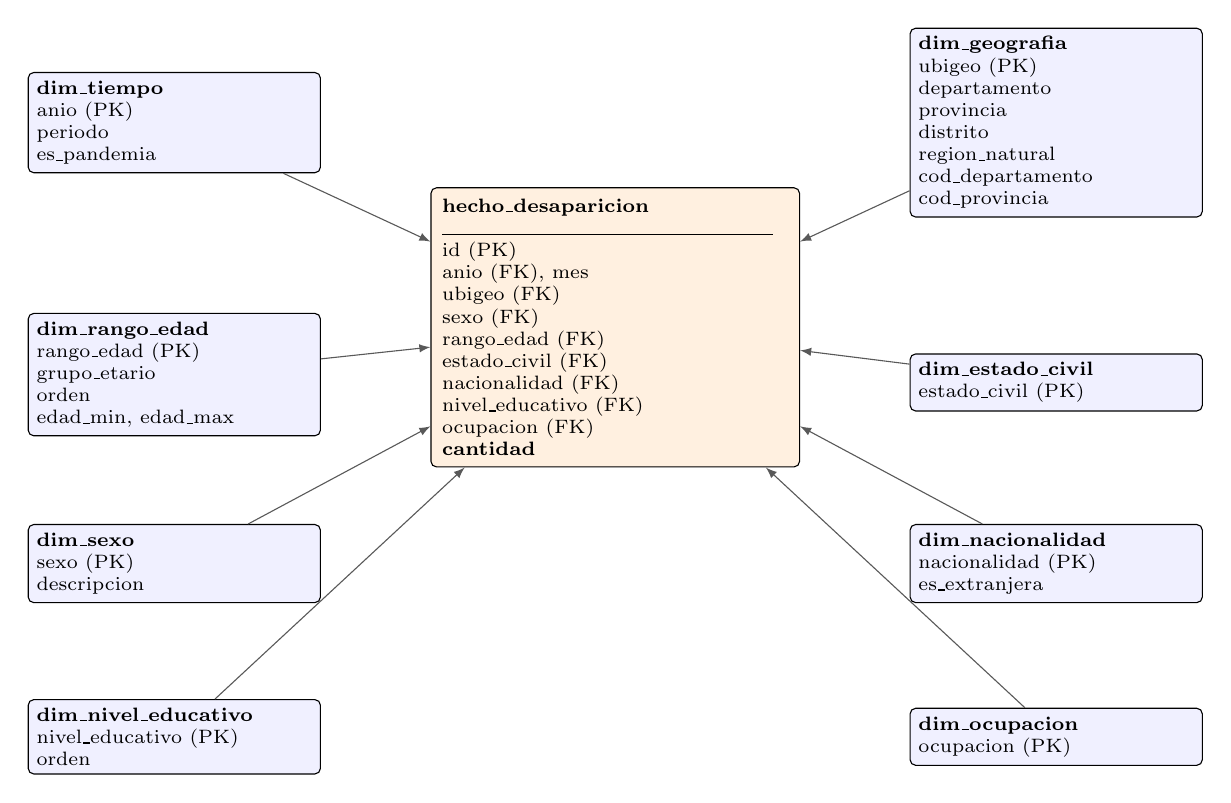
\begin{tikzpicture}[
  every node/.style={font=\scriptsize},
  dim/.style={draw, fill=blue!6, rounded corners=2pt, inner sep=3pt, align=left, text width=3.5cm},
  fac/.style={draw, fill=orange!12, rounded corners=2pt, inner sep=4pt, align=left, text width=4.4cm},
  link/.style={-latex, gray!70!black}
]
\node[fac] (hecho) at (0,0) {
  \textbf{hecho\_desaparicion}\\
  \rule{4.2cm}{0.2pt}\\
  id (PK)\\
  anio (FK), mes\\
  ubigeo (FK)\\
  sexo (FK)\\
  rango\_edad (FK)\\
  estado\_civil (FK)\\
  nacionalidad (FK)\\
  nivel\_educativo (FK)\\
  ocupacion (FK)\\
  \textbf{cantidad}
};
\node[dim] (tiempo) at (-5.6, 2.6) {\textbf{dim\_tiempo}\\ anio (PK)\\ periodo\\ es\_pandemia};
\node[dim] (geo)    at (5.6, 2.6)  {\textbf{dim\_geografia}\\ ubigeo (PK)\\ departamento\\ provincia\\ distrito\\ region\_natural\\ cod\_departamento\\ cod\_provincia};
\node[dim] (edad)   at (-5.6, -0.6) {\textbf{dim\_rango\_edad}\\ rango\_edad (PK)\\ grupo\_etario\\ orden\\ edad\_min, edad\_max};
\node[dim] (sexo)   at (-5.6, -3.0) {\textbf{dim\_sexo}\\ sexo (PK)\\ descripcion};
\node[dim] (civil)  at (5.6, -0.7) {\textbf{dim\_estado\_civil}\\ estado\_civil (PK)};
\node[dim] (nacion) at (5.6, -3.0) {\textbf{dim\_nacionalidad}\\ nacionalidad (PK)\\ es\_extranjera};
\node[dim] (nivel)  at (-5.6, -5.2) {\textbf{dim\_nivel\_educativo}\\ nivel\_educativo (PK)\\ orden};
\node[dim] (ocup)   at (5.6, -5.2) {\textbf{dim\_ocupacion}\\ ocupacion (PK)};
\draw[link] (tiempo) -- (hecho);
\draw[link] (geo) -- (hecho);
\draw[link] (edad) -- (hecho);
\draw[link] (sexo) -- (hecho);
\draw[link] (civil) -- (hecho);
\draw[link] (nacion) -- (hecho);
\draw[link] (nivel) -- (hecho);
\draw[link] (ocup) -- (hecho);
\end{tikzpicture}%
    }
    \par{\tiny PK: clave primaria. FK: clave foránea. Relación 1:N de dimensiones a hechos.}
    \column{0.24\textwidth}
    \scriptsize
    \textbf{1. Extraer.} \texttt{\textbackslash copy} carga las 93\,831 filas del CSV a
    \texttt{stg\_desaparicion}.\\[6pt]
    \textbf{2. Transformar.} Vacíos a NO ESPECIFICA, ubigeo a seis dígitos
    y una fila de catálogo por clave.\\[6pt]
    \textbf{3. Cargar.} Insertar dimensiones y después los hechos, con
    \texttt{cantidad > 0}, dentro de una transacción.\\[6pt]
    \textbf{Control.} El ubigeo 150121 tiene dos nombres.
    Agrupar por ubigeo antes de unir evita multiplicar filas.\\[6pt]
    \textcolor{verde}{\textbf{SUM(cantidad) = 121\,427}}\\
    Tanto en la base cargada como en la evidencia de restauración del dump.
  \end{columns}
  \fuente{Arquitectura: sql/01\_ddl.sql. Carga: sql/02\_etl.sql. Evidencia: pg-conteos.txt y pg-restauracion.txt.
    \enlace{captura-pg}{Conteos} · \enlace{evidencia-version}{Versión} · \enlace{evidencia-esquema}{Esquema} · \enlace{evidencia-consulta}{Consultas} · \enlace{evidencia-restauracion}{Restauración}.}
  \note{60 s. Definir grano, claves y relación 1:N. Explicar extraer, transformar y cargar. Mostrar el control del ubigeo sin cambiar la suma.}
\end{frame}
